\documentclass[10pt,a4paper]{article}
\usepackage[left=1.5cm,right=1.5cm,top=1.5cm,bottom=1.5cm]{geometry}
\usepackage[utf8]{inputenc}
\usepackage[german]{babel}
\usepackage{amsmath}
\usepackage{amsfonts}
\usepackage{amssymb}
\usepackage{amsthm}
\usepackage{graphicx}

\newenvironment{packed_enum}{
\begin{enumerate}
  \setlength{\itemsep}{1pt}
  \setlength{\parskip}{0pt}
  \setlength{\parsep}{0pt}
}{\end{enumerate}}
\newcommand{\abs}[1]{\ensuremath{\left\vert#1\right\vert}}
\begin{document}

\part*{Komplexe Funktionen}

\section{Vorletzte Seite schwarze FS kopieren}

\section{Allgemeines}
\subsection{Reihen}
Geometrische Reihe: $\frac{1}{1-q} = \sum\limits_{k=0}^\infty q^k\ \  |\ \  e^x = \sum\limits_{n=0}^\infty \frac{x^n}{n!} = 1+x+\frac{x^2}{2!} ... \ \ |\ \ sin(x)=\sum\limits_{n=0}^\infty (-1)^n \frac{x^{2n+1}}{(2n+1)!} = \frac{x}{1!} - \frac{x^3}{3!} + \frac{x^5}{5!}...$

$cos(x)=\sum\limits_{n=0}^\infty (-1)^n \frac{x^{2n}}{(2n)!} = \frac{x^0}{0!} - \frac{x^2}{2!} + \frac{x^4}{4!}...
 \ \ |\ \ sinh(x)=\sum\limits_{n=0}^\infty \frac{x^{2n+1}}{(2n+1)!}
  \ \ |\ \ cosh(x)=\sum\limits_{n=0}^\infty \frac{x^{2n}}{(2n)!}$

\subsection{Trigonometrie}
\[e^{iz} = cos(z)+i sin(z)
\ \ |\ \ e^z = e^x(cos(y)+i sin(y))
\ \ |\ \ cos(ix)=cosh(x)
\ \ |\ \ cosh(ix)=cos(x)\]
\[sin(x)=\frac{1}{2r}\left(e^{ix} - e^{-ix} \right)
\ \ |\ \ cosh(x)=\frac{e^x + e^{-x}}{2}
\ \ |\ \ sinh(x)=\frac{e^x - e^{-x}}{2}
\]

\section{Möbius Transformation}
\subsection{Bestimmen}
Transformation $w$ ist gegeben mit $T(z_1)=w_1$, $T(z_2)=w_2$ und $T(z_3)=w_3$ durch Doppelverhältnis:
\[
\frac{w-w_1}{w-w_2} : \frac{w_3-w_1}{w_3-w_2} = \frac{z-z_1}{z-z_2} : \frac{z_3-z_1}{z_3-z_2}
\Rightarrow
\frac{w-w_1}{w-w_2} = \frac{z-z_1}{z-z_2} \cdot \frac{z_3-z_2}{z_3-z_1}  \cdot \frac{w_3-w_1}{w_3-w_2}
\]
\begin{enumerate}
\item Zwei Punkte bestimmen die symmetrisch zu beiden Kreisen liegen: $(z_1 - z_0)(\overline{z}_2 - \overline{z}_0) = R^2$ für alle Gleichungen $|z - z_0| = R$ aufstellen, Gleichungssystem lösen
\item Transformation bestimmen: $T(a) = 0 \Rightarrow T_1(x) = x - a$, $T(b) = \infty \Rightarrow T_2(x) = \frac{x-a}{x-b}$, $T(c) = d \Rightarrow T(x) = \frac{x-a}{x-b} \cdot e = d$ erfüllen
\end{enumerate}
\subsection{Kreise}
Die Punkte $z_0$, $z_1$, $z_2$ und $z_3$ liegen auf einem verallgemeinerten Kreis wenn:
$\frac{z_0-z_1}{z_0-z_2} : \frac{z_3-z_1}{z_3-z_2} \in R$

Ist das Punktepaar $((0,0), (\infty, 0))$ symmetrisch so geht der Kreis im Bildraum durch den Ursprung und der Kreisradius $R$ sei $T(p)$ mit $p$ Randpunkt im Urbildraum auf Kreis.

\subsection{Konforme Funktion}
\[T(z) = k \frac{z-z1}{z-z2} \mbox{ mit } k \in R\setminus \lbrace 0 \rbrace\]

Wobei $T(z_1)=0, T(z_2)=\infty$. Konformitaet: $f'(z) \neq 0$

\section{Reihen}
\subsection{Taylorreihen}
\[
f(x) = A \int\limits_{start}^{end} \frac{1}{b - \xi} d\xi = \frac{A}{b+z_0} \int\limits_{start}^{end} \frac{1}{1- \frac{\xi - z_0}{b+z_0}} = A \sum\limits_{n=0}^\infty \frac{1}{(b+z_0)^{n+1}} \cdot \int\limits_{start}^{end} (\xi-z_0)^n d\xi
\]
Radius: $|$Entwicklungspunkt $ - $ Singularität$|$ - Kreise!

\subsection{Laurentreihen}
\begin{enumerate}
\item Bestimme Singularitäten
\item Hebe Hebbare Singularitäten
\item In Summe aus Hauptteilen ($ \frac{a}{(z-z_k)^k}$) und Nebenteilen ($ \frac{z-z_k}{a}$) umformen.
\end{enumerate}

\[
f(x)= \frac{A}{\xi - b}
= \frac{A}{\xi - z_0} \cdot \frac{1}{1 -\frac{(b-z_0)}{\xi - z_0}}
= \frac{A}{\xi - z_0} \cdot \sum\limits_{k=0}^\infty \left(\frac{b-z_0}{\xi - z_0}\right) ^k
\]

\subsubsection{Singularitäten}
Ringe $\rightarrow$ Pole
\begin{enumerate}
 \item Hebbar
 \item n-facher Pol
 \item Wesentliche Singularität
\end{enumerate}

\subsection{Residuen}
Berechnung ohne Laurent:
\begin{enumerate}
\item Polstelle 1. Ordnung: $Res(f,a) = \lim\limits_{z\rightarrow a} (z-a)f(z)$
\item Polstelle n. Ordnung: $Res(f,a) = \frac{1}{(n-1)!} \lim\limits_{z\rightarrow a} \left(\frac{d}{dz}\right)^{n-1} (z-a)^n f(z)$
\item $f(z)=\frac{g(z)}{h(z)} \,\,\,\, g(a) \neq 0, h(a) = 0, h'(a)\neq 0 \Rightarrow Res(f,a)=\frac{g(a)}{h(a)}$
\end{enumerate}

Mit Laurent:
$z_k$ seien die Singularitäten, $Res(f, a_k)$ die dazugehörigen Residuen wobei der $1$-te Hauptteil wie folgt aussieht: $\frac{Res(f, a_k)}{z-z_0}$

\subsection{Residuenkalkül}
\begin{itemize}
\item $\oint\limits_{K} f(z) dz = 2 \pi i \sum\limits_{z_k \neq 0} Res(f, a_k)$ wobei $Res(f, a_k)$ im Kreis
\item $\oint\limits_{-\infty}^{\infty} f(z) dz = 2 \pi i \sum\limits_{z_k \neq 0} Res(f, a_k)$ wobei $Im(Res(f, a_k)) \geq 0$
\item $\oint\limits_{0}^{\infty} f(z) dz = \pi i \sum\limits_{z_k \neq 0} Res(f, a_k)$
\end{itemize}

\subsection{Partialbruchzerlegung}
\begin{enumerate}
\item Residuen berechnen
\item Für alle Residuen: $f = \sum\limits_a \frac{Res(f, a)}{z-a}$
\end{enumerate}

\section{Kreisintegrale}
\begin{enumerate}
 \item Singularität liegt außerhalb oder auf dem Kreises - integral ist null
 \item Hebbare Singularität vorhanden - integral ist null
 \item Nichthebbare Singularität im Kreis:
 \begin{enumerate}
  \item Cauchysche Itegralformel $2 \pi i \cdot f(z_0) = \int \frac{f(z)}{(z-z_0)^n} dz$
  \item Verallg. Cauchysche Integralformel
 \end{enumerate}
\end{enumerate}

\section{Funktionseigenschaften}
\subsection{Holomorphie}
Eine Abbildung $f$ heißt holomorph wenn sie in jedem Punkt $z_0$ komplex differenzierbar ist. Dabei ist $f(z) = u(z) + v(z)i$ mit $u$ und $v$ reelle Funktionen.

Cauchy-Riemannsche DGL:
\[
\frac{\partial u}{\partial x} = \frac{\partial v}{\partial y}
\,\,\,\,\,\,\,\,\,\,\,\,\,\,\,\,\,\,\,\,\,\,\,\,
\frac{\partial u}{\partial y} = - \frac{\partial v}{\partial x}
\]

Schreibe: Da $u$ und $v$ stetig partiell differenzierbar sind ist $f$ holomorph.

Eine reelle Funktion muss konstant sein um holomorph zu sein.

Folgende Funktionen sind holomorph: polynomisch, trigonomisch, exponential, potenzreihen, rational.

Holomorphie impliziert harmonie.

\subsection{Harmonie}
Der Realteil einer Funktion ist harmonisch wenn die Funktion holomorph ist.

Eine Funktion $f=u + iv$ ist harmonisch wenn gilt: $f_{xx} + f_{yy} = 0$

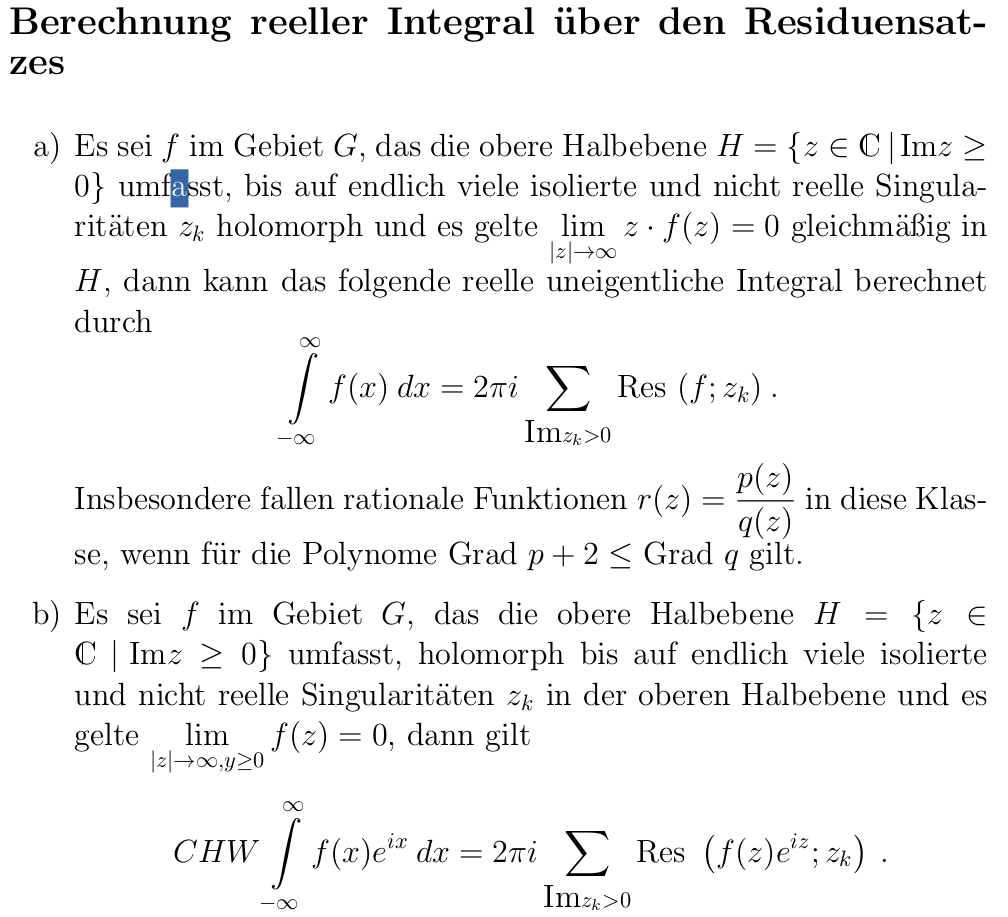
\includegraphics[scale=0.3]{kalk1}

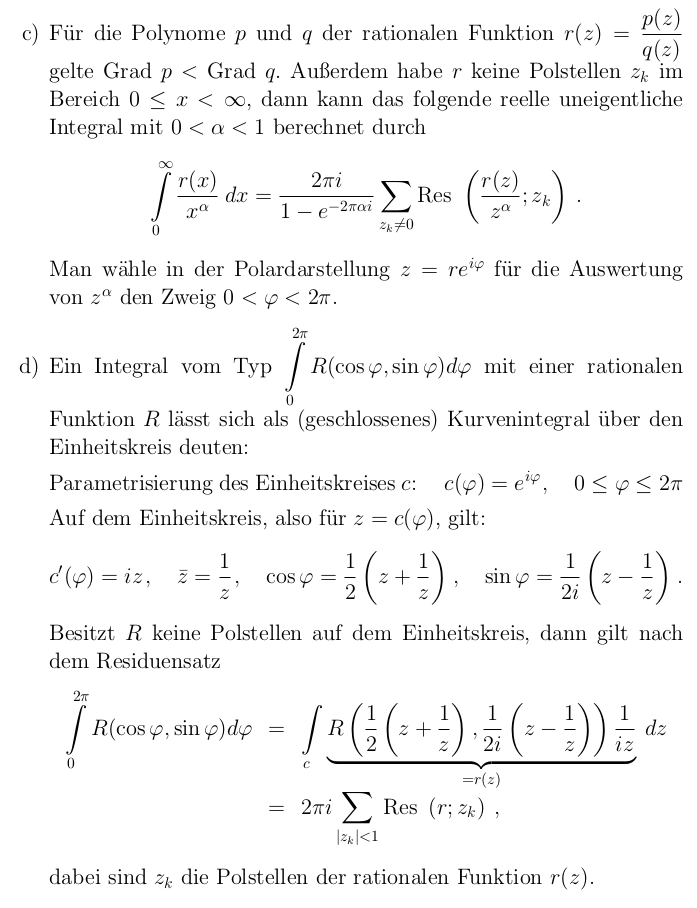
\includegraphics[scale=0.5]{kalk2}
\end{document}
